\documentclass[a4paper]{article}

\usepackage[T1]{fontenc}
\usepackage{newtxtext}     %TimesNewRoman
\usepackage[utf8]{inputenc} %UTF-8 Zeichensatz
\usepackage[ngerman]{babel} %Deutsch
\usepackage{lmodern}
\usepackage{pdfpages}
\usepackage{graphicx}   %Grafik einfuegen
\usepackage{float}      %Grafik fest positionieren
\usepackage{scrlayer-scrpage}   %Paket Kopf-/Fußzeile
\usepackage{csquotes}
\setcounter{tocdepth}{1}

\author{Jannik Ostermayer}

\begin{document}

\pagestyle{scrheadings}         %Kopf und Fußzeile mit Paket setzen
\clearpairofpagestyles          %Kopf & Fuß leeren
%footer
\ifoot{Jannik Ostermayer}
\cfoot{Matr.Nr. 672330}
\ofoot{\pagemark}

\begin{titlepage}

	\centering
	
\includegraphics[width=0.4\textwidth]{img/Logo_HS_Worms.png}\par\vspace{1cm}
	{\LARGE Entwicklung mobiler Anwendungen \par}
	\vspace{1.5cm}
	{\huge Projekt Fahrtenbuch\par}
	\vspace{0.3cm}
	{\huge Dokumentation\par}
	\vspace{2cm}
	{\Large Jannik Ostermayer\par}
	\vspace{1cm}
	{ Matrikelnummer 672330 \par}
	\vfill

% Bottom of the page
	{\large \today\par}

\end{titlepage}

\tableofcontents    %Inhaltsverzeichnis
\pagebreak                              %Seitenumbruch

\section{Idee}
Meine Idee ist eine Fahrtenbuchapp zum leichten Übertragen 
der Fahrten in ein physisches Fahrtenbuch.
Da es noch keine verifizierte Fahrtenbuchapp 
des Finanzamtes gibt und so auch keine Rechtssicherheit herrscht.
Zum leichteren übertragen sollte es auch eine Exportfunktion geben.
Da das übertragen in ein Fahrtenbuch zeitnahgeschehen (innerhalb der 
nächsten drei Tage) erfolgen muss sollte es auch Push Benachrichtungen
zur Erinnerung geben. 

\section{Beschreibung}
Diese App vereinfacht das führen eines Fahrtenbuches enorm. 
Alle Fahrten werden erfasst und du wirst Benachrichtigt, dass du dein 
Fahrtenahrtenbuch zeitnah führen kannst. 
Außerdem gibt es Export-Funktionen das du dir deine erfassetn Fahrten 
auch bequem auf deinem PC anschauen kannst.

\section{Zielgruppe}
Der potentielle Markt für eine Fahrtenbuch App erstreckt sich über alle
gewerblich genutzt Fahrzeuge in Deutschland. Das sind laut einer Statistik des KBA (Kraft Fahrt Bundesamtes)
aus dem Jahr 2017 64,4\% der zugelassenen Fahrzeuge in Deutschland. In absoluten Zahlen sind das 2.215.208
Gewerblich neu zugelassen Fahrzeuge. Meine App richtet sich aber spezial an Personen die einen
Firmenwagen fahren, wie Vertreter. Da es bei den Statistiken nur eine unterscheidung zwischen
geschäftlicher und privater Nutzung gibt, exestieren keine genauen Zahlen über Anzahl der Firmenwagen
unter den gewerblich genutzten Fahrzeugen. Man geht von ca 10\% der gesamten Fahrzeuge aus.
Laut KBA vom Stand 1. Januar 2018 gibt es in Deutschland 46,5 Millionen zugelessene PKWs.
Das bedeutet wenn man von 10\% ausgeht, gibt es in Deutschland 4,65 Millionen Firmenfahrzeuge.
Da sich meine App an Fahrer eines Firmenwagens richtet die Steuern sparen wollen und eine
erleichterung beim führen eines Fahrtenbuches suchen, trifft meine App auf einen potentiellen
Markt von 4,65 Millionen nutzern. Bei dem Führen von Fahrtenbüchern gibt es starke unterschiede
zwischen den Berufsgruppen, so muss zum Beispiel ein Handwerker für jede Fahrt den Grund der Fahrt angeben.
Dahingegen müssen Handelsvertreter und Kundendienstmonteure keinen Grund der Fahrt angeben, wenn der Grund
plausibel ist, hier reicht wenn der Kunde angegeben wird. Bei diesen Berufsgruppen die nicht alles angeben
müssen spricht man von einem \textit{erleichterten} Fahrtenbuch. In erste Linie soll sich meine App an Personen
die ein solches \textit{erleichtertes} Fahrtenbuch führen richten. Im nächsten Schritt, wenn meine App ausgebaut wird
würde ich auch gerne die anderen Berufsgruppen, die ein \textit{normales} Fahrtenbuch führen in
meine Zielgruppe mitaufnehmen.

%Grafik
%\begin{figure}[H]
%    \begin{center}
%        \includegraphics[width=12cm]{neuzulassung.jpg}
%        \caption{Verteilung der neuzugelassenen Fahrzeuge}
%        \label{Verteilung der neuzugelassenen Fahrzeuge}
%    \end{center}
%\end{figure}

\section{Marktanalyse}
Die meisten Apps im Play Store sollen ein Fahrtenbuch ersetzen. Diese bieten nur eingeschränkte
Funktionalitäten in der kostenlosen Version. Meist muss ein Abo abgeschlossen werden für 5-10€ pro Monat,
dafür gibt es meistens noch eine Web-Lösung und die möglichkeiten in Manipulationssichere Formate
zu expotieren. Exemplarisch werde ich ein paar Apps näher Analysieren.

\subsection{GPS Zeiterfassung + Fahrtenbuch}
Unter den Apps die ich analysiert habe wurde diese am häufigsten heruntergeladen mit über 100.000 Downloads.
Die App wurde durchschnittlich mit 4,6 Sternen bewertet bei 1.644 Rezesionen. Es gibt eine kostenlose Variante
und eine Pro Version für 9,99€.

\subsubsection{Design und Funktionalität}
Auf \ref{img:gps1} sehen Sie den Startbildschirm der App.
In der obere Hälfte des Bildschirm befinden sich Buttons \enquote{Abfahrt} und \enquote{Ankunft} um eine
Aufzeichnung zu starten und zu beende. Es gibt einen Button um den Kilometerstand des Autos zu korrigiert.
Außerdem kann man Kosten für das Auto und wie viel man getankt festhalten, was für meine App aber eher uninteressant ist.
In der unteren Hälfte des Bildschirm befindet sich eine Liste der erfassten fahrten und rechts unten ein optionen Button.
Wenn man auf eine erfasste fahrt klickt, siehe \ref{img:gps2}, werden neue Buttons in der oberen hälfte des Bildschirms geladen.
Man hat die Möglichkeit die Fahrt als \enquote{Dienst}, \enquote{Privat} oder \enquote{Sonst.} zu markieren, den Favoriten hinzuzufügen,
auf einer Karte anzuzeigen (siehe \ref{TODO}) oder das hinzuzufügen von Notizen oder eine Trennlinie in der Listen ansicht.

\begin{figure}[H]%zwei bilder nebeneinander
    \begin{minipage}[b]{.4\linewidth} % [b] => Ausrichtung an \caption
        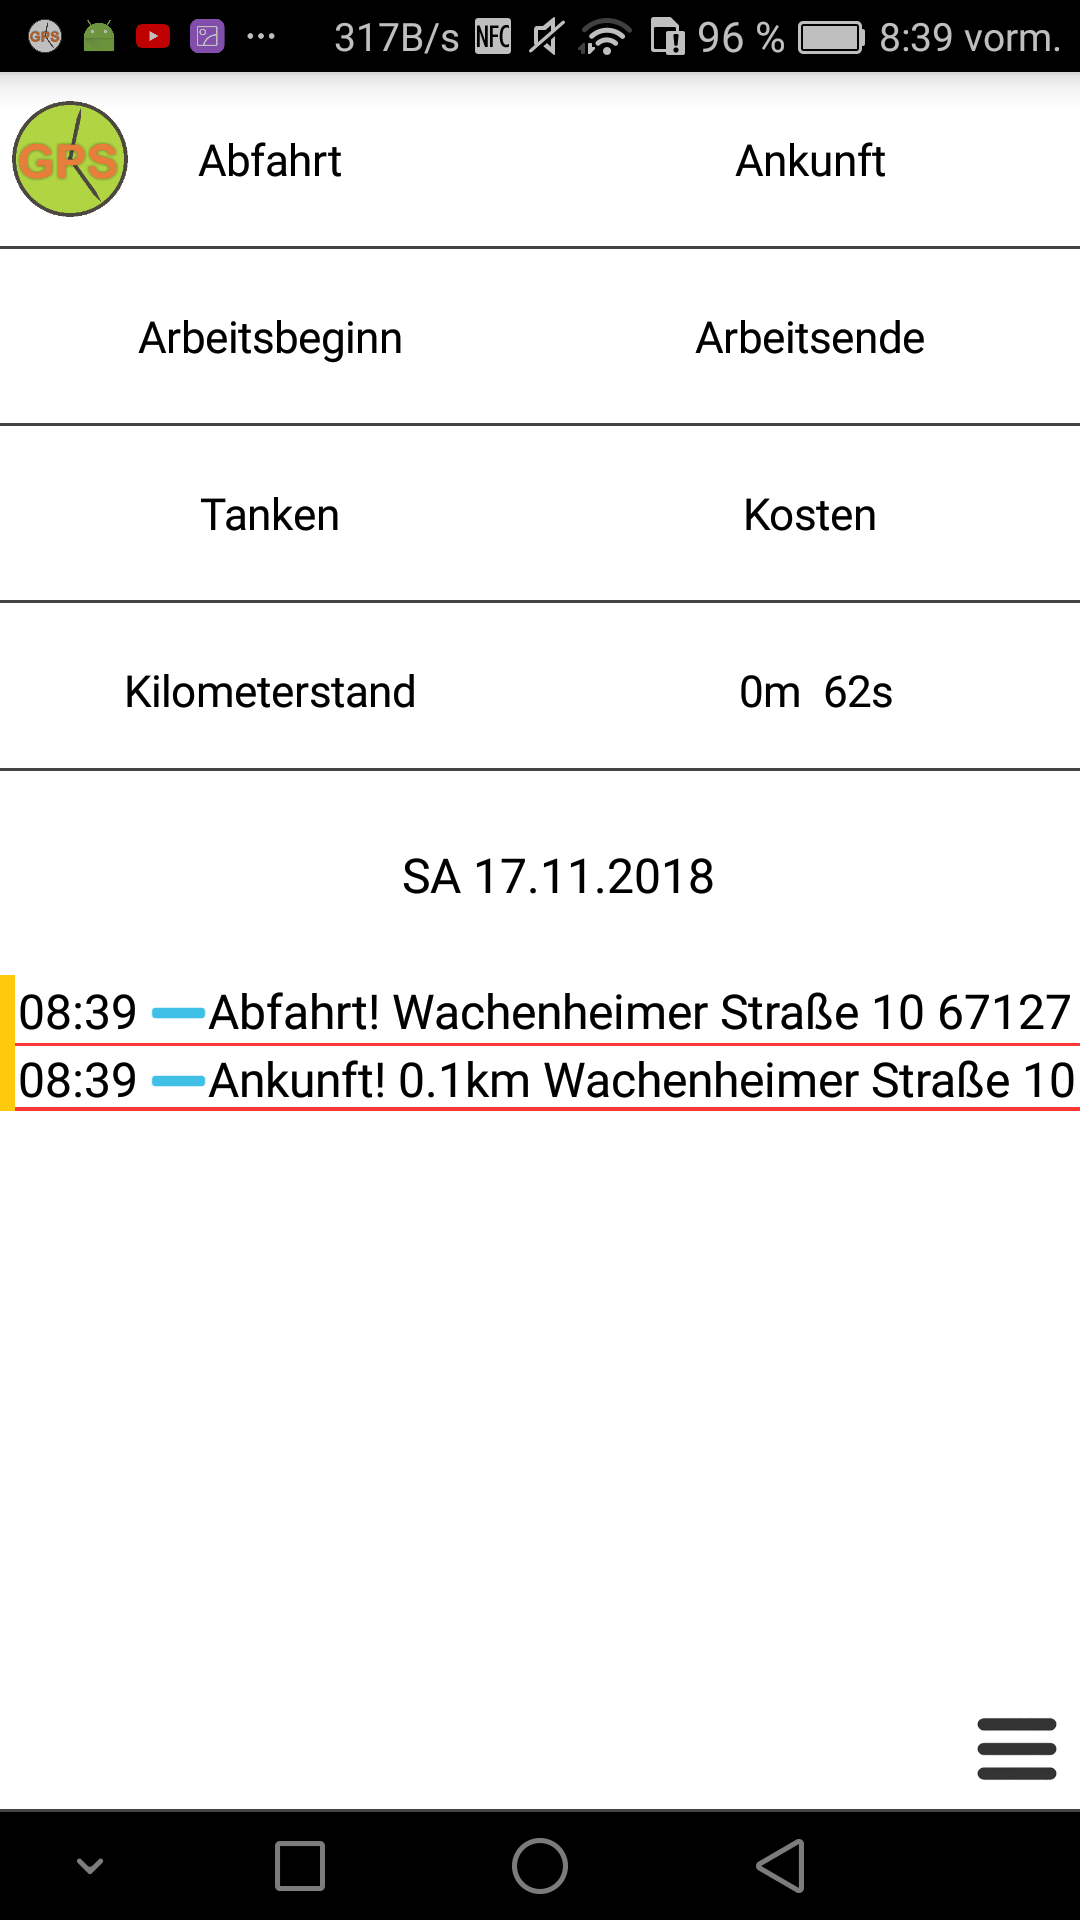
\includegraphics[scale=0.14]{gps1}
        \caption{\label{img:gps1}GPS Z+F Startbildschirm.}
    \end{minipage}
    \hspace{0.1\linewidth}% Abstand zwischen Bilder
    \begin{minipage}[b]{.4\linewidth} % [b] => Ausrichtung an \caption
        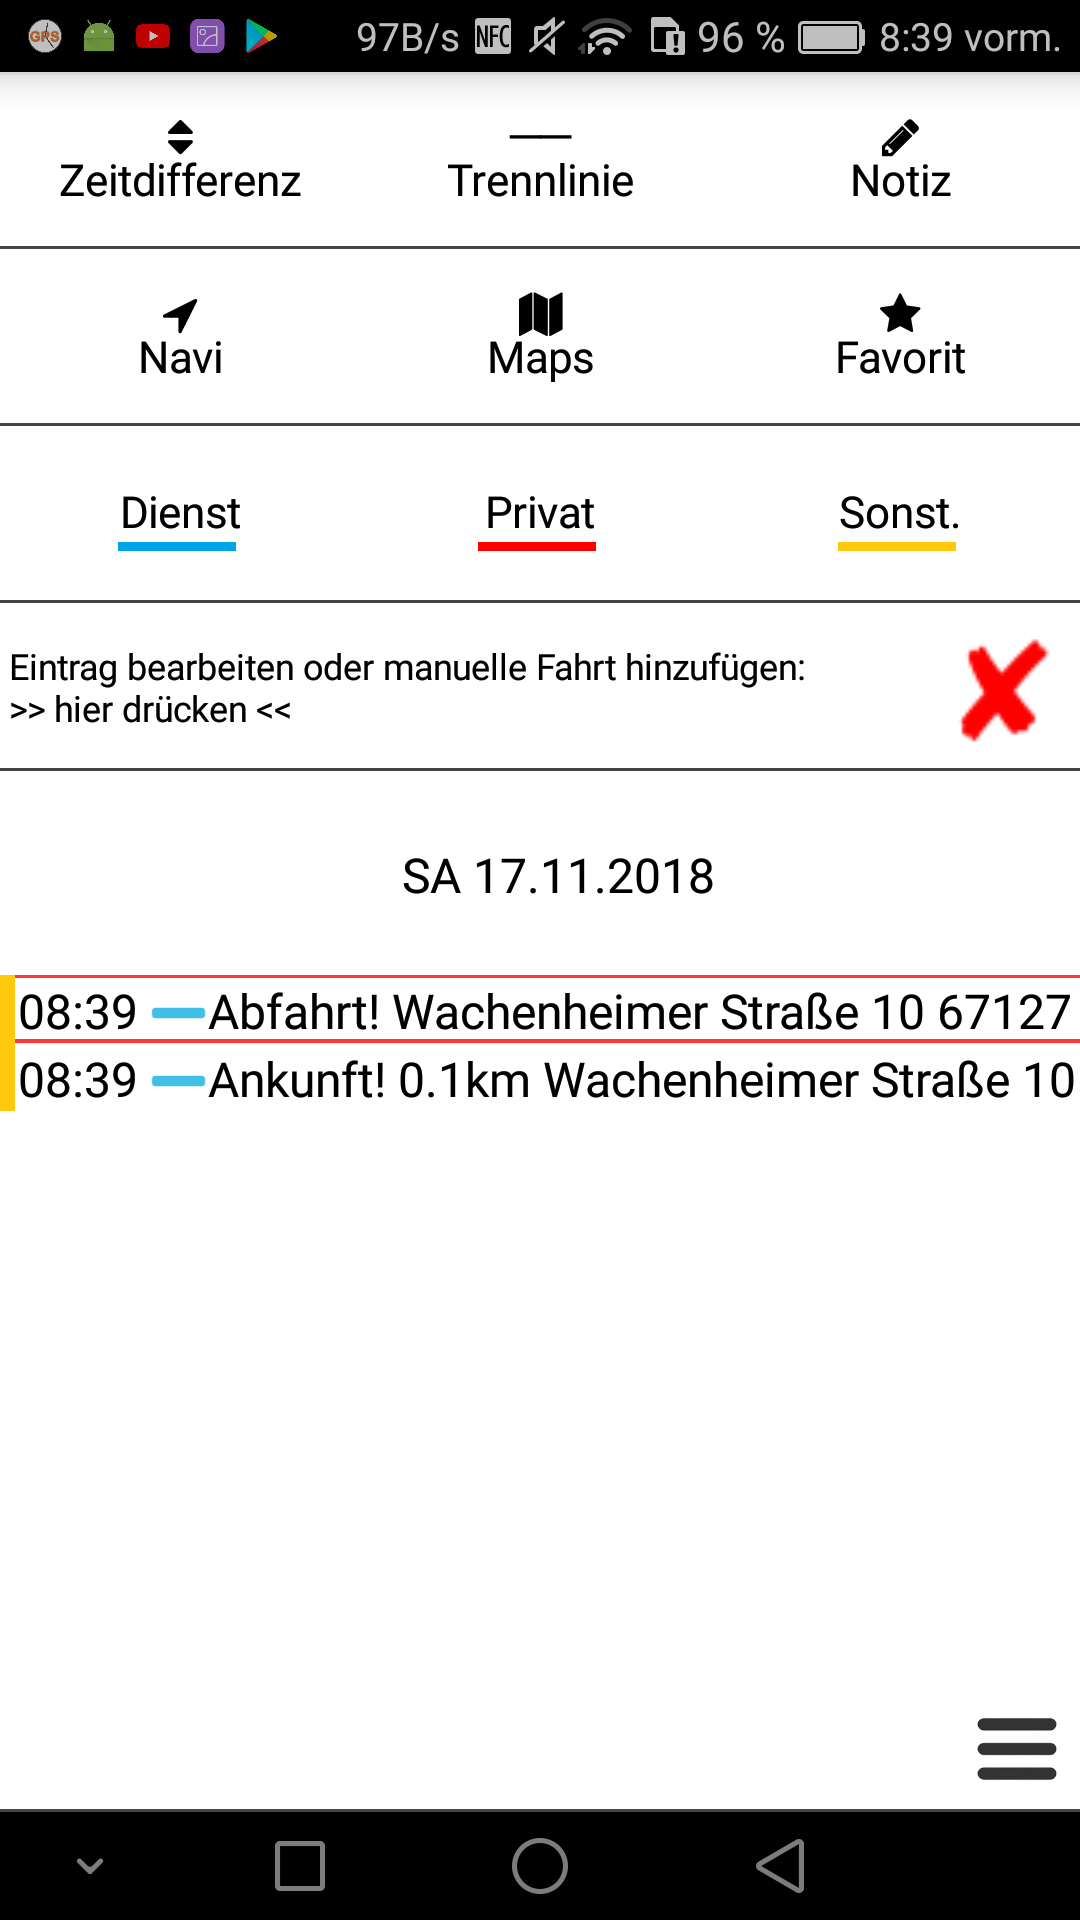
\includegraphics[scale=0.14]{gps2}
        \caption{\label{img:gps2}GPS Z+F Fahrt ausgewählt.}
    \end{minipage}
\end{figure}

\subsubsection{Kommentare im Play Store}
\begin{enumerate}
    \item Der automatische Start und Ende der Aufzeichnungen ist sehr gut.
    \item Nicht Finanzamt konform da Änderungen nicht nachvollziehbar sind (nur in der Pro Version).
    \item Bedienung nicht induitiv.
\end{enumerate}

\subsubsection{Fazit}
Diese App ist im punkte Funktionalität woll die beste Lösung die es ohne Abo gibt. Aber designtechnisch
sehe ich noch Verbesserungspotential. Die Hälfte des Bildschirms besteht nur aus Buttons, die Liste
der erfassten Fahrten ist sehr klein und der optionen Button im rechten unteren Eck entspricht nicht
den Style-Guides. Gut ist die Ansicht der Routen auf einer Karte.

\subsection{kfz fahrtenbuch}
durchschnittliche Bewertung 2,9 Sterne bei 52 Rezessionen und 10.000+ Downloads.
Wird in einem ABo zusammen mit einer Cloud Lösung angeboten. Viele Nutzer kritisieren das
Preis-Leistungsverhältnis der Cloud Lösung.

\subsection{SquareTrip}
durchschnittlich 4,1 Sterne bei 118 Rezesionen und 10.000+ Downloads
Die meisten Bewertungen sind zufrieden mit der App

\subsection{Driverslog Pro 2 - Fahrtenbuch}
Nur eine Testlizenz
App ist abgestürzt und nicht mehr gestartet
durschnittliche Bewerung von 3,9 Sternen bei 60 Rezensionen und 5.000+ Downnloads.

\section{Bedarfsanalyse}

\section{Features}
\subsection{Anforderungen}
\begin{enumerate}
	\item Die Fahrtenbuch Daten sollen in einer Datenbank auf dem Handy gespeichert werden.
	\item Alle Einträge der Datenbank sollen in einer Liste dargestellt werden.
	\item Die Liste enthält die Information Zeit, Zweck, Start, Ziel
	\item Die Liste kann man nach Datum sotieren.
	\item Der Benutzer kann in der Liste suchen.
	\item Der Benutzer kann auf ein Element der Liste klicken und bekommt eine Detailansicht.
	\item Die App speichert die Daten in der Form wir die vom Finanzamt anerkannten Fahrtenbücher.
	\item Die App muss per GPS erfassen wenn der Benutzer losfährt und automatisch Start-, Endpunkt und Entfernung bestimmen und diese eintragen.
	\item Die App muss den Benutzer Auffordern fehlende Information, wie \enquote{Zweck der Fahrt nachzutragen}.
	\item Der Benutzer muss Fahrten in der App händisch eintragen können.
	\item Der Benutzer muss alle Fahrtenbuch Daten expotieren können als PDF oder HTML(bzw. Jason).
	\item Die App soll automatisch starten wenn das Handy per Blutooth mit dem Auto gekoppelt wird.
	\item Der Benutzer soll Einträge bearbeiten können.
	\item Der Benutzer soll Einträge löschen können.
\end{enumerate}

\section{User Stories, Personas}

\section{Mockuop, Wireframe}

\section{UML-Diagramme}

\section{Code Dokumentation}

\section{Fazit}
%Input(einleitung.tex) ->einleitung.tex einbinden

\end{document}